%iffalse
\let\negmedspace\undefined
\let\negthickspace\undefined
\documentclass[journal,12pt,onecolumn]{IEEEtran}
\usepackage{cite}
\usepackage{amsmath,amssymb,amsfonts,amsthm}
\usepackage{algorithmic}
\usepackage{graphicx}
\usepackage{textcomp}
\usepackage{xcolor}
\usepackage{txfonts}
\usepackage{listings}
\usepackage{enumitem}
\usepackage{mathtools}
\usepackage{gensymb}
\usepackage{comment}
\usepackage[breaklinks=true]{hyperref}
\usepackage{tkz-euclide} 
\usepackage{listings}
\usepackage{gvv}
\def\inputGnumericTable{}                                 
\usepackage[latin1]{inputenc}                              
\usepackage{color}                                         
\usepackage{array}                                        
\usepackage{longtable}                                     
\usepackage{calc}                                          
\usepackage{multirow}                                      
\usepackage{hhline}                                        
\usepackage{ifthen}                                        
\usepackage{lscape}
\newtheorem{theorem}{Theorem}[section]
\newtheorem{problem}{Problem}
\newtheorem{proposition}{Proposition}[section]
\newtheorem{lemma}{Lemma}[section]
\newtheorem{corollary}[theorem]{Corollary}
\newtheorem{example}{Example}[section]
\newtheorem{definition}[problem]{Definition}
\newcommand{\BEQA}{\begin{eqnarray}}
\newcommand{\EEQA}{\end{eqnarray}}
\newcommand{\define}{\stackrel{\triangle}{=}}
\theoremstyle{remark}
\newtheorem{rem}{Remark}
\graphicspath{ {./Figures/} }
\usepackage{float} % For the [H] float option
\usepackage{textcomp}
\usepackage{multicol}

\begin{document}

\begin{enumerate}[start=1, label=Q.\arabic*]

% Question 1
\item Two independent random variables $X$ and $Y$ are uniformly distributed in the interval $[-1,1]$. The probability that $\max[X, Y]$ is less than $1/2$ is

\begin{enumerate}
    \begin{multicols}{4}
    \item $3/4$
    \item $9/16$
    \item $1/4$
    \item $2/3$
    \end{multicols}
\end{enumerate}
\hfill{\brak{\text{GATE EE 2012}}}

% Question 2
\item If $x=\sqrt{-1}$, then the value of $x^{x}$ is

\begin{enumerate}
    \begin{multicols}{4}
    \item $e^{-\pi/2}$
    \item $e^{\pi/2}$
    \item $x$
    \item $1$
    \end{multicols}
\end{enumerate}
\hfill{\brak{\text{GATE EE 2012}}}

% Question 3
\item Given $f(z)=\frac{1}{z+1}-\frac{2}{z+3}$. If C is a counterclockwise path in the z-plane such that $\abs{z+1}=1$, the value of $\frac{1}{2\pi j}\oint_{c}f(z)dz$ is

\begin{enumerate}
    \begin{multicols}{4}
    \item $-2$
    \item $-1$
    \item $1$
    \item $2$
    \end{multicols}
\end{enumerate}
\hfill{\brak{\text{GATE EE 2012}}}

% Question 4
\item In the circuit shown below, the current through the inductor is
\begin{figure}[H]
    \centering
    \includegraphics[width=0.4\columnwidth]{Figures/q4.png}
    \caption{}
\end{figure}

\hfill{\brak{\text{GATE EE 2012}}}
\begin{enumerate}
\begin{multicols}{4}
    
    \item $\frac{2}{1+j}A$
    \item $\frac{-1}{1+j}A$
    \item $\frac{1}{1+j}A$
    \item $0 A$
    \end{multicols}

\end{enumerate}

% Question 5
\item The impedance looking into nodes 1 and 2 in the given circuit is
\begin{figure}[H]
    \centering
    \includegraphics[width=0.4\columnwidth]{q5}
    \caption{}
\end{figure}

\begin{enumerate}
    \begin{multicols}{2}
    \item $50~\ohm$
    \item $100~\ohm$
    \item $5~k\ohm$
    \item $10.1~k\ohm$
    \end{multicols}
\end{enumerate}
\hfill{\brak{\text{GATE EE 2012}}}

% Question 6
\item A system with transfer function $G(s)=\frac{\brak{s^{2}+9}\brak{s+2}}{\brak{s+1}\brak{s+3}\brak{s+4}}$ is excited by $\sin(\omega t)$. The steady-state output of the system is zero at

\begin{enumerate}
    \begin{multicols}{2}
    \item $\omega=1~\text{rad/s}$
    \item $\omega=2~\text{rad/s}$
    \item $\omega=3~\text{rad/s}$
    \item $\omega=4~\text{rad/s}$
    \end{multicols}
\end{enumerate}
\hfill{\brak{\text{GATE EE 2012}}}

% Question 7
\item In the sum of products function $f(X,Y,Z)=\sum(2,3,4,5)$, the prime implicants are

\begin{enumerate}
    \item $\overline{X}Y$, $X\overline{Y}$
    \item $\overline{X}Y$, $X\overline{Y}\overline{Z}$, $X\overline{Y}Z$
    \item $\overline{X}Y\overline{Z}$, $\overline{X}YZ$, $X\overline{Y}$
    \item $\overline{X}Y\overline{Z}$, $\overline{X}YZ$, $X\overline{Y}\overline{Z}$, $X\overline{Y}Z$
\end{enumerate}
\hfill{\brak{\text{GATE EE 2012}}}

% Question 8
\item If $x[n]=(1/3)^{\abs{n}}-(1/2)^{n}u[n]$, then the region of convergence \brak{ROC} of its Z-transform in the Z-plane will be

\begin{enumerate}
    \begin{multicols}{2}
    \item $\frac{1}{3}<\abs{z}<3$
    \item $\frac{1}{3}<\abs{z}<\frac{1}{2}$
    \item $\frac{1}{2}<\abs{z}<3$
    \item $\frac{1}{3}<\abs{z}$
    \end{multicols}
\end{enumerate}
\hfill{\brak{\text{GATE EE 2012}}}

% Question 9
\item The bus admittance matrix of a three-bus three-line system is $Y=j\myvec{-13 & 10 & 5 \\ 10 & -18 & 10 \\ 5 & 10 & -13}$. If each transmission line between the two buses is represented by an equivalent $\pi$-network, the magnitude of the shunt susceptance of the line connecting bus 1 and 2 is

\begin{enumerate}
    \begin{multicols}{4}
    \item $4$
    \item $2$
    \item $1$
    \item $0$
    \end{multicols}
\end{enumerate}
\hfill{\brak{\text{GATE EE 2012}}}

% Question 10
\item The slip of an induction motor normally does not depend on

\begin{enumerate}
    \begin{multicols}{2}
    \item rotor speed
    \item synchronous speed
    \item shaft torque
    \item core-loss component
    \end{multicols}
\end{enumerate}
\hfill{\brak{\text{GATE EE 2012}}}

% Question 11
\item A two-phase load draws the following phase currents: $i_{1}(t)=I_{m}\sin(\omega t-\phi_{1})$, $i_{2}(t)=I_{m}\cos(\omega t-\phi_{2})$. These currents are balanced if $\phi_{1}$ is equal to

\begin{enumerate}
    \begin{multicols}{2}
    \item $-\phi_{2}$
    \item $\phi_{2}$
    \item $(\pi/2-\phi_{2})$
    \item $(\pi/2+\phi_{2})$
    \end{multicols}
\end{enumerate}
\hfill{\brak{\text{GATE EE 2012}}}

% Question 12
\item A periodic voltage waveform observed on an oscilloscope across a load is shown. A permanent magnet moving coil \brak{PMMC} meter connected across the same load reads
\begin{figure}[H]
    \centering
    \includegraphics[width=0.4\columnwidth]{Figures/q12.png}
    \caption{}
\end{figure}

\begin{enumerate}
    \begin{multicols}{4}
    \item $4$ V
    \item $5$ V
    \item $8$ V
    \item $10$ V
    \end{multicols}
\end{enumerate}
\hfill{\brak{\text{GATE EE 2012}}}

% Question 13
\item The bridge method commonly used for finding mutual inductance is

\begin{enumerate}
    \begin{multicols}{2}
    \item Heaviside Campbell bridge
    \item Schering bridge
    \item De Sauty bridge
    \item Wien bridge
    \end{multicols}
\end{enumerate}
\hfill{\brak{\text{GATE EE 2012}}}

% Question 14
\item With initial condition $x(1)=0.5$, the solution of the differential equation $t\frac{dx}{dt}+x=t$ is

\begin{enumerate}
    \begin{multicols}{2}
    \item $x=t-\frac{1}{2}$
    \item $x=t^{2}-\frac{1}{2}$
    \item $x=\frac{t^{2}}{2}$
    \item $x=\frac{t}{2}$
    \end{multicols}
\end{enumerate}
\hfill{\brak{\text{GATE EE 2012}}}

% Question 15
\item The unilateral Laplace transform of $f(t)$ is $\frac{1}{s^{2}+s+1}$. The unilateral Laplace transform of $t f(t)$ is

\begin{enumerate}
    \item $-\frac{s}{\brak{s^{2}+s+1}^{2}}$
    \item $-\frac{2s+1}{\brak{s^{2}+s+1}^{2}}$
    \item $\frac{s}{\brak{s^{2}+s+1}^{2}}$
    \item $\frac{2s+1}{\brak{s^{2}+s+1}^{2}}$
\end{enumerate}
\hfill{\brak{\text{GATE EE 2012}}}

% Question 16
\item The average power delivered to an impedance $(4-j3)~\ohm$ by a current $5\cos(100\pi t+100)$ A is

\begin{enumerate}
    \begin{multicols}{2}
    \item $44.2$ W
    \item $50$ W
    \item $62.5$ W
    \item $125$ W
    \end{multicols}
\end{enumerate}
\hfill{\brak{\text{GATE EE 2012}}}

% Question 17
\item In the following figure, $C_{1}$ and $C_{2}$ are ideal capacitors. $C_{1}$ has been charged to $12$ V before the ideal switch S is closed at $t=0$. The current i(t) for all t is
\begin{figure}[H]
    \centering
    \includegraphics[width=0.3\columnwidth]{Figures/q17.png}
    \caption{}
\end{figure}

\begin{enumerate}
    \begin{multicols}{2}
    \item zero
    \item a step function
    \item an exponentially decaying function
    \item an impulse function
    \end{multicols}
\end{enumerate}
\hfill{\brak{\text{GATE EE 2012}}}

% Question 18
\item The i-v characteristics of the diode in the circuit given below are
$i=\begin{cases}\frac{v-0.7}{500}A, & v\ge0.7~V\\ 0~A, & v<0.7~V\end{cases}$
The current in the circuit is
\begin{figure}[H]
    \centering
    \includegraphics[width=0.2\columnwidth]{Figures/q18.png}
    \caption{}
\end{figure}

\begin{enumerate}
    \begin{multicols}{2}
    \item $10$ mA
    \item $9.3$ mA
    \item $6.67$ mA
    \item $6.2$ mA
    \end{multicols}
\end{enumerate}
\hfill{\brak{\text{GATE EE 2012}}}

% Question 19
\item The output Y of a 2-bit comparator is logic 1 whenever the 2-bit input A is greater than the 2-bit input B. The number of combinations for which the output is logic 1, is

\begin{enumerate}
    \begin{multicols}{4}
    \item $4$
    \item $6$
    \item $8$
    \item $10$
    \end{multicols}
\end{enumerate}
\hfill{\brak{\text{GATE EE 2012}}}

% Question 20
\item Consider the given circuit.
\begin{figure}[H]
    \centering
    \includegraphics[width=0.4\columnwidth]{Figures/q20.png}
    \caption{}
\end{figure}
In this circuit, the race around

\begin{enumerate}
    \item does not occur
    \item occurs when $CLK=0$
    \item occurs when $CLK=1$ and $A=B=1$
    \item occurs when $CLK=1$ and $A=B=0$
\end{enumerate}
\hfill{\brak{\text{GATE EE 2012}}}

% Question 21
\item The figure shows a two-generator system supplying a load of $P_{D}=40$ MW, connected at bus 2.
\begin{figure}[H]
    \centering
    \includegraphics[width=0.5\columnwidth]{Figures/q21.png}
    \caption{}
\end{figure}
The fuel cost of generators $G_{1}$ and $G_{2}$ are: $C_{1}(P_{G1})=10,000~\text{Rs/MWh}$ and $C_{2}(P_{G2})=12,500~\text{Rs/MWh}$ and the loss in the line is $P_{loss(pu)}=0.5P_{G1(pu)}^{2}$, where the loss coefficient is specified in pu on a 100 MVA base. The most economic power generation schedule in MW is

\begin{enumerate}
    \begin{multicols}{2}
    \item $P_{G1}=20$, $P_{G2}=22$
    \item $P_{G1}=22$, $P_{G2}=20$
    \item $P_{G1}=20$, $P_{G2}=20$
    \item $P_{G1}=0$, $P_{G2}=40$
    \end{multicols}
\end{enumerate}
\hfill{\brak{\text{GATE EE 2012}}}

% Question 22
\item The sequence components of the fault current are as follows: $I_{positive}=j1.5~\text{pu}$, $I_{negative}=-j0.5~\text{pu}$, $I_{zero}=-j1~\text{pu}$. The type of fault in the system is

\begin{enumerate}
    \begin{multicols}{4}
    \item LG
    \item LL
    \item LLG
    \item LLLG
    \end{multicols}
\end{enumerate}
\hfill{\brak{\text{GATE EE 2012}}}

% Question 23
\item A half-controlled single-phase bridge rectifier is supplying an R-L load. It is operated at a firing angle $\alpha$ and the load current is continuous. The fraction of cycle that the freewheeling diode conducts is

\begin{enumerate}
    \begin{multicols}{2}
    \item $1/2$
    \item $(1-\alpha/\pi)$
    \item $\alpha/2\pi$
    \item $\alpha/\pi$
    \end{multicols}
\end{enumerate}
\hfill{\brak{\text{GATE EE 2012}}}

% Question 24
\item The typical ratio of latching current to holding current in a 20 A thyristor is

\begin{enumerate}
    \begin{multicols}{4}
    \item $5.0$
    \item $2.0$
    \item $1.0$
    \item $0.5$
    \end{multicols}
\end{enumerate}
\hfill{\brak{\text{GATE EE 2012}}}

% Question 25
\item For the circuit shown in the figure, the voltage and current expressions are $v(t)=E_{1}\sin(\omega t)+E_{3}\sin(3\omega t)$ and $i(t)=I_{1}\sin(\omega t-\phi_{1})+I_{3}\sin(3\omega t-\phi_{3})+I_{5}\sin(5\omega t)$. The average power measured by the Wattmeter is
\begin{figure}[H]
    \centering
    \includegraphics[width=0.4\columnwidth]{Figures/q25.png}
    \caption{}
\end{figure}

\begin{enumerate}
    \item $\frac{1}{2}E_{1}I_{1}\cos\phi_{1}$
    \item $\frac{1}{2}[E_{1}I_{1}\cos\phi_{1}+E_{1}I_{3}\cos\phi_{3}+E_{1}I_{5}]$
    \item $\frac{1}{2}[E_{1}I_{1}\cos\phi_{1}+E_{3}I_{3}\cos\phi_{3}]$
    \item $\frac{1}{2}[E_{1}I_{1}\cos\phi_{1}+E_{3}I_{1}\cos\phi_{1}]$
\end{enumerate}
\hfill{\brak{\text{GATE EE 2012}}}

% Question 26
\item Given that $A=\myvec{-5 & -3 \\ 2 & 0}$ and $I=\myvec{1 & 0 \\ 0 & 1}$, the value of $A^{3}$ is

\begin{enumerate}
    \begin{multicols}{2}
    \item $15A+12 I$
    \item $19 A+30 I$
    \item $17A+15 I$
    \item $17A+21 I$
    \end{multicols}
\end{enumerate}
\hfill{\brak{\text{GATE EE 2012}}}

% Question 27
\item The maximum value of $f(x)=x^{3}-9x^{2}+24x+5$ in the interval $[1, 6]$ is

\begin{enumerate}
    \begin{multicols}{4}
    \item $21$
    \item $25$
    \item $41$
    \item $46$
    \end{multicols}
\end{enumerate}
\hfill{\brak{\text{GATE EE 2012}}}

% Question 28
\item If $V_{A}-V_{B}=6~V,$ then $V_{C}-V_{D}$ is
\begin{figure}[H]
    \centering
    \includegraphics[width=0.6\columnwidth]{Figures/q28.png}
    \caption{}
\end{figure}

\begin{enumerate}
    \begin{multicols}{4}
    \item $-5$ V
    \item $2$ V
    \item $3$ V
    \item $6$ V
    \end{multicols}
\end{enumerate}
\hfill{\brak{\text{GATE EE 2012}}}

% Question 29
\item The voltage gain $A_{v}$ of the circuit shown below is
\begin{figure}[H]
    \centering
    \includegraphics[width=0.4\columnwidth]{Figures/q29.png}
    \caption{}
\end{figure}

\begin{enumerate}
    \begin{multicols}{4}
    \item $\abs{A_{v}}\approx200$
    \item $\abs{A_{v}}\approx100$
    \item $\abs{A_{v}}\approx20$
    \item $\abs{A_{v}}\approx10$
    \end{multicols}
\end{enumerate}
\hfill{\brak{\text{GATE EE 2012}}}
% Question 30
\item The state transition diagram for the logic circuit shown is
\begin{figure}[H]
    \centering
    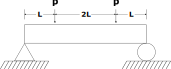
\includegraphics[width=0.4\columnwidth]{Figures/q30.png}
    \caption{}
\end{figure}

\begin{enumerate}
\item 
    \begin{figure}[H]
    \centering
    \includegraphics[width=0.4\columnwidth]{Figures/q30A.png}
    \caption{}
    \end{figure}
    \item 
    \begin{figure}[H]
    \centering
    \includegraphics[width=0.4\columnwidth]{Figures/q30B.png}
    \caption{}
    \end{figure}
    \item 
    \begin{figure}[H]
    \centering
    \includegraphics[width=0.4\columnwidth]{Figures/q30C.png}
    \caption{}
    \end{figure}
    \item 
    \begin{figure}[H]
    \centering
    \includegraphics[width=0.4\columnwidth]{Figures/q30D.png}
    \caption{}
    \end{figure}
\end{enumerate}
\hfill{\brak{\text{GATE EE 2012}}}

% Question 31
\item Let $y[n]$ denote the convolution of $h[n]$ and $g[n]$, where $h[n]=(1/2)^{n}u[n]$ and $g[n]$ is a causal sequence. If $y[0]=1$ and $y[1]=1/2$, then $g[1]$ equals

\begin{enumerate}
    \begin{multicols}{4}
    \item $0$
    \item $1/2$
    \item $1$
    \item $3/2$
    \end{multicols}
\end{enumerate}
\hfill{\brak{\text{GATE EE 2012}}}

% Question 32
\item The circuit shown is a
\begin{figure}[H]
    \centering
    \includegraphics[width=0.4\columnwidth]{Figures/q32.png}
    \caption{}
\end{figure}

\begin{enumerate}
    \item low pass filter with $f_{3dB}=\frac{1}{(R_{1}+R_{2})C}\text{rad/s}$
    \item high pass filter with $f_{3dB}=\frac{1}{R_{1}C}\text{rad/s}$
    \item low pass filter with $f_{3dB}=\frac{1}{R_{1}C}\text{rad/s}$
    \item high pass filter with $f_{3dB}=\frac{1}{(R_{1}+R_{2})C}\text{rad/s}$
\end{enumerate}
\hfill{\brak{\text{GATE EE 2012}}}

% Question 33
\item For the system shown below, $S_{D1}$ and $S_{D2}$ are complex power demands at bus 1 and bus 2 respectively. If $\abs{V_{2}}=1\text{pu}$, the VAR rating of the capacitor \brak{Q_{G2}} connected at bus 2 is
\begin{figure}[H]
    \centering
    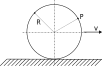
\includegraphics[width=0.5\columnwidth]{Figures/q33.png}
    \caption{}
\end{figure}

\begin{enumerate}
    \begin{multicols}{4}
    \item $0.2$ pu
    \item $0.268$ pu
    \item $0.312$ pu
    \item $0.4$ pu
    \end{multicols}
\end{enumerate}
\hfill{\brak{\text{GATE EE 2012}}}

% Question 34
\item A cylindrical rotor generator delivers $0.5$ pu power in the steady-state to an infinite bus through a transmission line of reactance $0.5$ pu. The generator no-load voltage is $1.5$ pu and the infinite bus voltage is $1$ pu. The inertia constant of the generator is $5$ MW-s/MVA and the generator reactance is $1$ pu. The critical clearing angle, in degrees, for a three-phase dead short circuit fault at the generator terminal is

\begin{enumerate}
    \begin{multicols}{4}
    \item $53.5$
    \item $60.2$
    \item $70.8$
    \item $79.6$
    \end{multicols}
\end{enumerate}
\hfill{\brak{\text{GATE EE 2012}}}

% Question 35
\item In the circuit shown, an ideal switch S is operated at $100$ kHz with a duty ratio of $50\%$. Given that $\Delta i_{c}$ is $1.6$ A peak-to-peak and $I_{0}$ is $5$ A dc, the peak current in S is
\begin{figure}[H]
    \centering
    \includegraphics[width=0.5\columnwidth]{Figures/q35.png}
    \caption{}
\end{figure}

\begin{enumerate}
    \begin{multicols}{4}
    \item $6.6$ A
    \item $5.0$ A
    \item $5.8$ A
    \item $4.2$ A
    \end{multicols}
\end{enumerate}
\hfill{\brak{\text{GATE EE 2012}}}

% Question 36
\item A 220 V, 15 kW, 1000 rpm shunt motor with armature resistance of $0.25~\ohm$, has a rated line current of 68 A and a rated field current of 2.2 A. The change in field flux required to obtain a speed of 1600 rpm while drawing a line current of 52.8 A and a field current of 1.8 A is

\begin{enumerate}
    \begin{multicols}{2}
    \item $18.18\%$ increase
    \item $18.18\%$ decrease
    \item $36.36\%$ increase
    \item $36.36\%$ decrease
    \end{multicols}
\end{enumerate}
\hfill{\brak{\text{GATE EE 2012}}}

% Question 37
\item A fair coin is tossed till a head appears for the first time. The probability that the number of required tosses is odd, is

\begin{enumerate}
    \begin{multicols}{4}
    \item $1/3$
    \item $1/2$
    \item $2/3$
    \item $3/4$
    \end{multicols}
\end{enumerate}
\hfill{\brak{\text{GATE EE 2012}}}

% Question 38
\item The direction of vector A is radially outward from the origin, with $\abs{A}=k r^{n}$ where $r^{2}=x^{2}+y^{2}+z^{2}$ and k is a constant. The value of n for which $\nabla\cdot A=0$ is

\begin{enumerate}
    \begin{multicols}{4}
    \item $-2$
    \item $2$
    \item $1$
    \item $0$
    \end{multicols}
\end{enumerate}
\hfill{\brak{\text{GATE EE 2012}}}

% Question 39
\item Consider the differential equation $\frac{d^{2}y(t)}{dt^{2}}+2\frac{dy(t)}{dt}+y(t)=\delta(t)$ with $y(t)|_{t=0^{-}}=-2$ and $\frac{dy}{dt}|_{t=0^{-}}=0$. The numerical value of $\frac{dy}{dt}|_{t=0^{+}}$ is

\begin{enumerate}
    \begin{multicols}{4}
    \item $-2$
    \item $-1$
    \item $0$
    \item $1$
    \end{multicols}
\end{enumerate}
\hfill{\brak{\text{GATE EE 2012}}}

% Question 40
\item Assuming both the voltage sources are in phase, the value of R for which maximum power is transferred from circuit A to circuit B is
\begin{figure}[H]
    \centering
    \includegraphics[width=0.5\columnwidth]{Figures/q40.png}
    \caption{}
\end{figure}

\begin{enumerate}
    \begin{multicols}{2}
    \item $0.8~\ohm$
    \item $1.4~\ohm$
    \item $2~\ohm$
    \item $2.8~\ohm$
    \end{multicols}
\end{enumerate}
\hfill{\brak{\text{GATE EE 2012}}}

% Question 41
\item The state variable description of an LTI system is given by
$\myvec{\dot{x}_{1} \\ \dot{x}_{2} \\ \dot{x}_{3}}=\myvec{0 & a_{1} & 0 \\ 0 & 0 & a_{2} \\ a_{3} & 0 & 0}\myvec{x_{1} \\ x_{2} \\ x_{3}}+\myvec{0 \\ 0 \\ 1}u$
$y=\myvec{1 & 0 & 0}\myvec{x_{1} \\ x_{2} \\ x_{3}}$
where y is the output and u is the input. The system is controllable for

\begin{enumerate}
    \item $a_{1}\ne0$, $a_{2}=0$, $a_{3}\ne0$
    \item $a_{1}=0$, $a_{2}\ne0$, $a_{3}\ne0$
    \item $a_{1}=0$, $a_{2}\ne0$, $a_{3}=0$
    \item $a_{1}\ne0$, $a_{2}\ne0$, $a_{3}=0$
\end{enumerate}
\hfill{\brak{\text{GATE EE 2012}}}

% Question 42
\item The Fourier transform of a signal $h(t)$ is $H(j\omega)=(2\cos\omega)(\sin 2\omega)/\omega$. The value of $h(0)$ is

\begin{enumerate}
    \begin{multicols}{4}
    \item $1/4$
    \item $1/2$
    \item $1$
    \item $2$
    \end{multicols}
\end{enumerate}
\hfill{\brak{\text{GATE EE 2012}}}

% Question 43
\item The feedback system shown below oscillates at $2~\text{rad/s}$ when
\begin{figure}[H]
    \centering
    \includegraphics[width=0.6\columnwidth]{Figures/q41.png}
    \caption{}
\end{figure}

\begin{enumerate}
    \begin{multicols}{2}
    \item $K=2$ and $a=0.75$
    \item $K=3$ and $a=0.75$
    \item $K=4$ and $a=0.5$
    \item $K=2$ and $a=0.5$
    \end{multicols}
\end{enumerate}
\hfill{\brak{\text{GATE EE 2012}}}

% Question 44
\item The input $x(t)$ and output $y(t)$ of a system are related as $y(t)=\int_{-\infty}^{t}x(\tau)\cos(3\tau)d\tau$. The system is

\begin{enumerate}
    \item time-invariant and stable
    \item stable and not time-invariant
    \item time-invariant and not stable
    \item not time-invariant and not stable
\end{enumerate}
\hfill{\brak{\text{GATE EE 2012}}}

% Question 45
\item An analog voltmeter uses external multiplier settings. With a multiplier setting of $20~k\ohm$, it reads 440 V and with a multiplier setting of $80~k\ohm$, it reads 352 V. For a multiplier setting of $40~k\ohm$, the voltmeter reads

\begin{enumerate}
    \begin{multicols}{4}
    \item $371$ V
    \item $383$ V
    \item $394$ V
    \item $406$ V
    \end{multicols}
\end{enumerate}
\hfill{\brak{\text{GATE EE 2012}}}

% Question 46
\item The locked rotor current in a 3-phase, star connected 15 kW, 4-pole, 230 V, 50 Hz induction motor at rated conditions is 50 A. Neglecting losses and magnetizing current, the approximate locked rotor line current drawn when the motor is connected to a 236 V, 57 Hz supply is

\begin{enumerate}
    \begin{multicols}{4}
    \item $58.5$ A
    \item $45.0$ A
    \item $42.7$ A
    \item $55.6$ A
    \end{multicols}
\end{enumerate}
\hfill{\brak{\text{GATE EE 2012}}}

% Question 47
\item A single phase 10 kVA, 50 Hz transformer with 1 kV primary winding draws 0.5 A and 55 W, at rated voltage and frequency, on no load. A second transformer has a core with all its linear dimensions $\sqrt{2}$ times the corresponding dimensions of the first transformer. The core material and lamination thickness are the same in both transformers. The primary windings of both the transformers have the same number of turns. If a rated voltage of 2 kV at 50 Hz is applied to the primary of the second transformer, then the no load current and power, respectively, are

\begin{enumerate}
    \begin{multicols}{2}
    \item 0.7 A, 77.8 W
    \item 0.7 A, 155.6 W
    \item 1 A, 110 W
    \item 1 A, 220 W
    \end{multicols}
\end{enumerate}
\hfill{\brak{\text{GATE EE 2012}}}

\vspace{1cm}
\textbf{Common Data for Questions 48 and 49:}\\
In the 3-phase inverter circuit shown, the load is balanced and the gating scheme is 180\degree-conduction mode. All the switching devices are ideal.
\begin{figure}[H]
    \centering
    \includegraphics[width=0.5\columnwidth]{Figures/comp1.png}
    \caption{}
\end{figure}
% Question 48
\item The rms value of load phase voltage is

\begin{enumerate}
    \begin{multicols}{4}
    \item 106.1 V
    \item 141.4 V
    \item 212.2 V
    \item 282.8 V
    \end{multicols}
\end{enumerate}
\hfill{\brak{\text{GATE EE 2012}}}

% Question 49
\item If the dc bus voltage Vd =300 V, the power consumed by 3-phase load is

\begin{enumerate}
    \begin{multicols}{4}
    \item 1.5 kW
    \item 2.0 kW
    \item 2.5 kW
    \item 3.0 kW
    \end{multicols}
\end{enumerate}
\hfill{\brak{\text{GATE EE 2012}}}

\vspace{1cm}
\textbf{Common Data for Questions 50 and 51:}\\
With 10 V dc connected at port A in the linear nonreciprocal two-port network shown below, the following were observed:
\begin{enumerate}
    \item[i] 1 $\ohm$ connected at port B draws a current of 3 A
    \item[ii] 2.5 $\ohm$ connected at port B draws a current of 2 A
\end{enumerate}
\begin{figure}[H]
    \centering
    \includegraphics[width=0.4\columnwidth]{Figures/comp2.png}
    \caption{}
\end{figure}

% Question 50
\item For the same network, with 6 V dc connected at port A, 1 $\ohm$ connected at port B draws 7/3 A. If 8 V dc is connected to port A, the open circuit voltage at port B is

\begin{enumerate}
    \begin{multicols}{4}
    \item 6 V
    \item 7 V
    \item 8 V
    \item 9 V
    \end{multicols}
\end{enumerate}
\hfill{\brak{\text{GATE EE 2012}}}

% Question 51
\item With 10 V dc connected at port A, the current drawn by 7 $\ohm$ connected at port B is

\begin{enumerate}
    \begin{multicols}{4}
    \item 3/7 A
    \item 5/7 A
    \item 1 A
    \item 9/7 A
    \end{multicols}
\end{enumerate}
\hfill{\brak{\text{GATE EE 2012}}}

\vspace{1cm}
\textbf{Statement for Linked Answer Questions 52 and 53:}\\
In the circuit shown, the three voltmeter readings are $V_{1} = 220V$, $V_{2} = 122V$, $V_{3} = 136V$.
\begin{figure}[H]
    \centering
    \includegraphics[width=0.4\columnwidth]{Figures/comp3.png}
    \caption{}
\end{figure}

% Question 52
\item The power factor of the load is

\begin{enumerate}
    \begin{multicols}{4}
    \item 0.45
    \item 0.50
    \item 0.55
    \item 0.60
    \end{multicols}
\end{enumerate}
\hfill{\brak{\text{GATE EE 2012}}}

% Question 53
\item If $R_{L} = 5~\ohm$, the approximate power consumption in the load is

\begin{enumerate}
    \begin{multicols}{4}
    \item 700 W
    \item 750 W
    \item 800 W
    \item 850 W
    \end{multicols}
\end{enumerate}
\hfill{\brak{\text{GATE EE 2012}}}

\vspace{1cm}
\textbf{Statement for Linked Answer Questions 54 and 55:}\\
\begin{center}
    
The transfer function of a compensator is given as $G_{c}(s) = \frac{s+a}{s+b}$.
\end{center}
% Question 54
\item $G_{c}(s)$ is a lead compensator if

\begin{enumerate}
    \begin{multicols}{2}
    \item a = 1, b = 2
    \item a = 3, b = 2
    \item a = -3, b = -1
    \item a = 3, b = 1
    \end{multicols}
\end{enumerate}
\hfill{\brak{\text{GATE EE 2012}}}

% Question 55
\item The phase of the above lead compensator is maximum at

\begin{enumerate}
    \begin{multicols}{2}
    \item $\sqrt{2}$ rad/s
    \item $\sqrt{3}$ rad/s
    \item $\sqrt{6}$ rad/s
    \item $1/\sqrt{3}$ rad/s
    \end{multicols}
\end{enumerate}
\hfill{\brak{\text{GATE EE 2012}}}

\vspace{1cm}
\textbf{{General Aptitude (GA) Questions}}\\
% Question 56
\item One of the parts (A, B, C, D) in the sentence given below contains an ERROR. Which one of the following is INCORRECT?
\textit{I requested that he should be given the driving test today instead of tomorrow.}

\begin{enumerate}
    \item requested that
    \item should be given
    \item the driving test
    \item instead of tomorrow
\end{enumerate}
\hfill{\brak{\text{GATE EE 2012}}}

% Question 57
\item If $(1.001)^{1259} = 3.52$ and $(1.001)^{2062} = 7.85$, then $(1.001)^{3321}=$

\begin{enumerate}
    \begin{multicols}{4}
    \item 2.23
    \item 4.33
    \item 11.37
    \item 27.64
    \end{multicols}
\end{enumerate}
\hfill{\brak{\text{GATE EE 2012}}}

% Question 58
\item Choose the most appropriate alternative from the options given below to complete the following sentence: \textit{If the tired soldier wanted to lie down, he \underline{\hspace{2cm}} the mattress out on the balcony.}

\begin{enumerate}
    \item should take
    \item shall take
    \item should have taken
    \item will have taken
\end{enumerate}
\hfill{\brak{\text{GATE EE 2012}}}

% Question 59
\item Choose the most appropriate word from the options given below to complete the following sentence: \textit{Given the seriousness of the situation that he had to face, his \underline{\hspace{2cm}} was impressive.}

\begin{enumerate}
    \begin{multicols}{2}
    \item beggary
    \item nomenclature
    \item jealousy
    \item nonchalance
    \end{multicols}
\end{enumerate}
\hfill{\brak{\text{GATE EE 2012}}}

% Question 60
\item Which one of the following options is the closest in meaning to the word given below? \textit{Latitude}

\begin{enumerate}
    \begin{multicols}{2}
    \item Eligibility
    \item Freedom
    \item Coercion
    \item Meticulousness
    \end{multicols}
\end{enumerate}
\hfill{\brak{\text{GATE EE 2012}}}

% Question 61
\item A and B are friends. They decide to meet between 1 PM and 2 PM on a given day. There is a condition that whoever arrives first will not wait for the other for more than 15 minutes. The probability that they will meet on that day is

\begin{enumerate}
    \begin{multicols}{4}
    \item 1/4
    \item 1/16
    \item 7/16
    \item 9/16
    \end{multicols}
\end{enumerate}
\hfill{\brak{\text{GATE EE 2012}}}

% Question 62
\item One of the legacies of the Roman legions was discipline. In the legions, military law prevailed and discipline was brutal. Discipline on the battlefield kept units obedient, intact and fighting, even when the odds and conditions were against them. Which one of the following statements best sums up the meaning of the above passage?

\begin{enumerate}
    \item Thorough regimentation was the main reason for the efficiency of the Roman legions even in adverse circumstances.
    \item The legions were treated inhumanly as if the men were animals.
    \item Discipline was the armies’ inheritance from their seniors.
    \item The harsh discipline to which the legions were subjected to led to the odds and conditions being against them.
\end{enumerate}
\hfill{\brak{\text{GATE EE 2012}}}

% Question 63
\item Raju has 14 currency notes in his pocket consisting of only Rs. 20 notes and Rs. 10 notes. The total money value of the notes is Rs. 230. The number of Rs. 10 notes that Raju has is

\begin{enumerate}
    \begin{multicols}{4}
    \item 5
    \item 6
    \item 9
    \item 10
    \end{multicols}
\end{enumerate}
\hfill{\brak{\text{GATE EE 2012}}}

% Question 64
\item There are eight bags of rice looking alike, seven of which have equal weight and one is slightly heavier. The weighing balance is of unlimited capacity. Using this balance, the minimum number of weighings required to identify the heavier bag is

\begin{enumerate}
    \begin{multicols}{4}
    \item 2
    \item 3
    \item 4
    \item 8
    \end{multicols}
\end{enumerate}
\hfill{\brak{\text{GATE EE 2012}}}

% Question 65
\item The data given in the following table summarizes the monthly budget of an average household.
\begin{table}[H]
\centering
\begin{tabular}{|l|c|}
\hline
\textbf{Category} & \textbf{Amount (Rs.)} \\
\hline
Food & 4000 \\
Clothing & 1200 \\
Rent & 2000 \\
Savings & 1500 \\
Other expenses & 1800 \\
\hline
\end{tabular}
\caption*{}
\label{tab:budget}
\end{table}
The approximate percentage of the monthly budget NOT spent on savings is

\begin{enumerate}
    \begin{multicols}{4}
    \item 10\%
    \item 14\%
    \item 81\%
    \item 86\%
    \end{multicols}
\end{enumerate}
\hfill{\brak{\text{GATE EE 2012}}}

\end{enumerate}
\end{document}